\chapter{Konzeption}
\label{Konzeption}
Nachfolgend wird die Konzeption des Projekts beschrieben. 
Die Kommunikation wird nachrichtenbasiert umgesetzt. Dies bedeutet, dass die Komponenten des verteilten Systems kommunizieren, indem sie sich Nachrichten übermitteln können. Die Steuerung der Kommunikation wird primär von den als Master 
(siehe \ref{glossar}) ausgewählten Komponenten umgesetzt. Als Provider wird ein angepasster Webserver eingesetzt, die Verbindung der einzelnen Komponenten zueinander geschieht über WebSockets. Der Webserver basiert auf dem Javascript-Framework Node.js. \\


\section{Brute Force-Algorithmus}
\label{ideeBruteForce}
Primäres Ziel des Projektes ist das Entschlüsseln eines vorgegebenen Passwortes. Das zu entschlüsselnde Passwort wird vor der Berechnung vom Benutzer eingegeben. Das eingetragene Passwort wird dann durch eine Hashfunktion geleitet. Der entstandene Hash wird gespeichert und dient als Zielbedingung der folgenden Berechnung. \\
Nun beginnt der eigentliche Angriff. Zu Beginn wird eine sogenannte \enquote{Dictionary-Attack} vorgenommen. Dies bedeutet, dass ein Wörterbuch mit häufig genutzten Passwörtern als Basis des Angriffs genutzt wird. Die eingetragenen Passwörter werden ebenfalls der Reihe nach gehasht und der berechnete Hash mit dem Zielhash verglichen. \\
 Durch die vorangestellte Attacke auf Basis von häufig benutzten Passwörtern wird die Effizienz des verteilten Systems verbessert. Der folgende Auszug aus der Passwortliste  verdeutlicht das Prinzip eines Dictionaries. \\
\texttt{Dictionary:}
\begin{lstlisting}[basicstyle=\ttfamily,numbers=left,numberstyle=\footnotesize\ttfamily,backgroundcolor=\color{sourcegray}]
	LOVE123
	LOVEME1
	Lamont1
	Leasowes2
	Lemon123
	Liberty
	Lindsay
	Lizard
	Love21
	MASTER
	MORIAH07
	MOSS18
	Madeline
	Margaret
	Master
	Matthew
	Maxwell
	Mellon
	Merlot
	Metallic
	Michael
\end{lstlisting}



Bleibt die Dictionary-Attack erfolglos, wir der BruteForce-Angriff durchgeführt. \\
Die erste Idee war es, dass der steuernde Rechner alle möglichen Passwörter berechnet und in einem Array ablegen wird. Dabei sollten die Passwörter eine statische Länge besitzen. Das Muster der möglichen Passwörter sollte wie folgt aufgebaut werden: \\
\texttt{Muster der zu berechnenden Passwörter:}
\begin{lstlisting}[basicstyle=\ttfamily,numbers=left,numberstyle=\footnotesize\ttfamily,backgroundcolor=\color{sourcegray}]
	Array passwordsUPPER = 
		[A*****,
	 	B*****,
	 	C*****,
	 	D*****,
	 	...
	]
	
	
	Array passwordsLOWER = 
		[a*****,
	 	b*****,
	 	c*****,
	 	d*****,
		...
	]
	
	

	Array passwordsNUM = 
		[1*****,
	 	2*****,
	 	3*****,
	 	4*****,
		...
	]
\end{lstlisting}

Die exemplarische Darstellung soll die geplante Aufteilung verdeutlichen. Die hier dargestellte feste Länge der Passwörter auf 6 Zeichen dient als Beispiel. \\

In der Praxis werden alle möglichen Passwörter probiert, begonnen mit Passwörtern der Länge = 1. Wird kein Passwort ermittelt, so werden Passwörter der Länge n+1 erzeugt. Abbildung \ref{fig:schemaBruteForce} stellt das Konzept zur Berechnung aller möglichen Passwörter dar. Der genaue Algorithmus dazu wird in Kapitel \ref{implementation} ausführlicher beschrieben. \\
\begin{figure}[!ht]
	\centering
		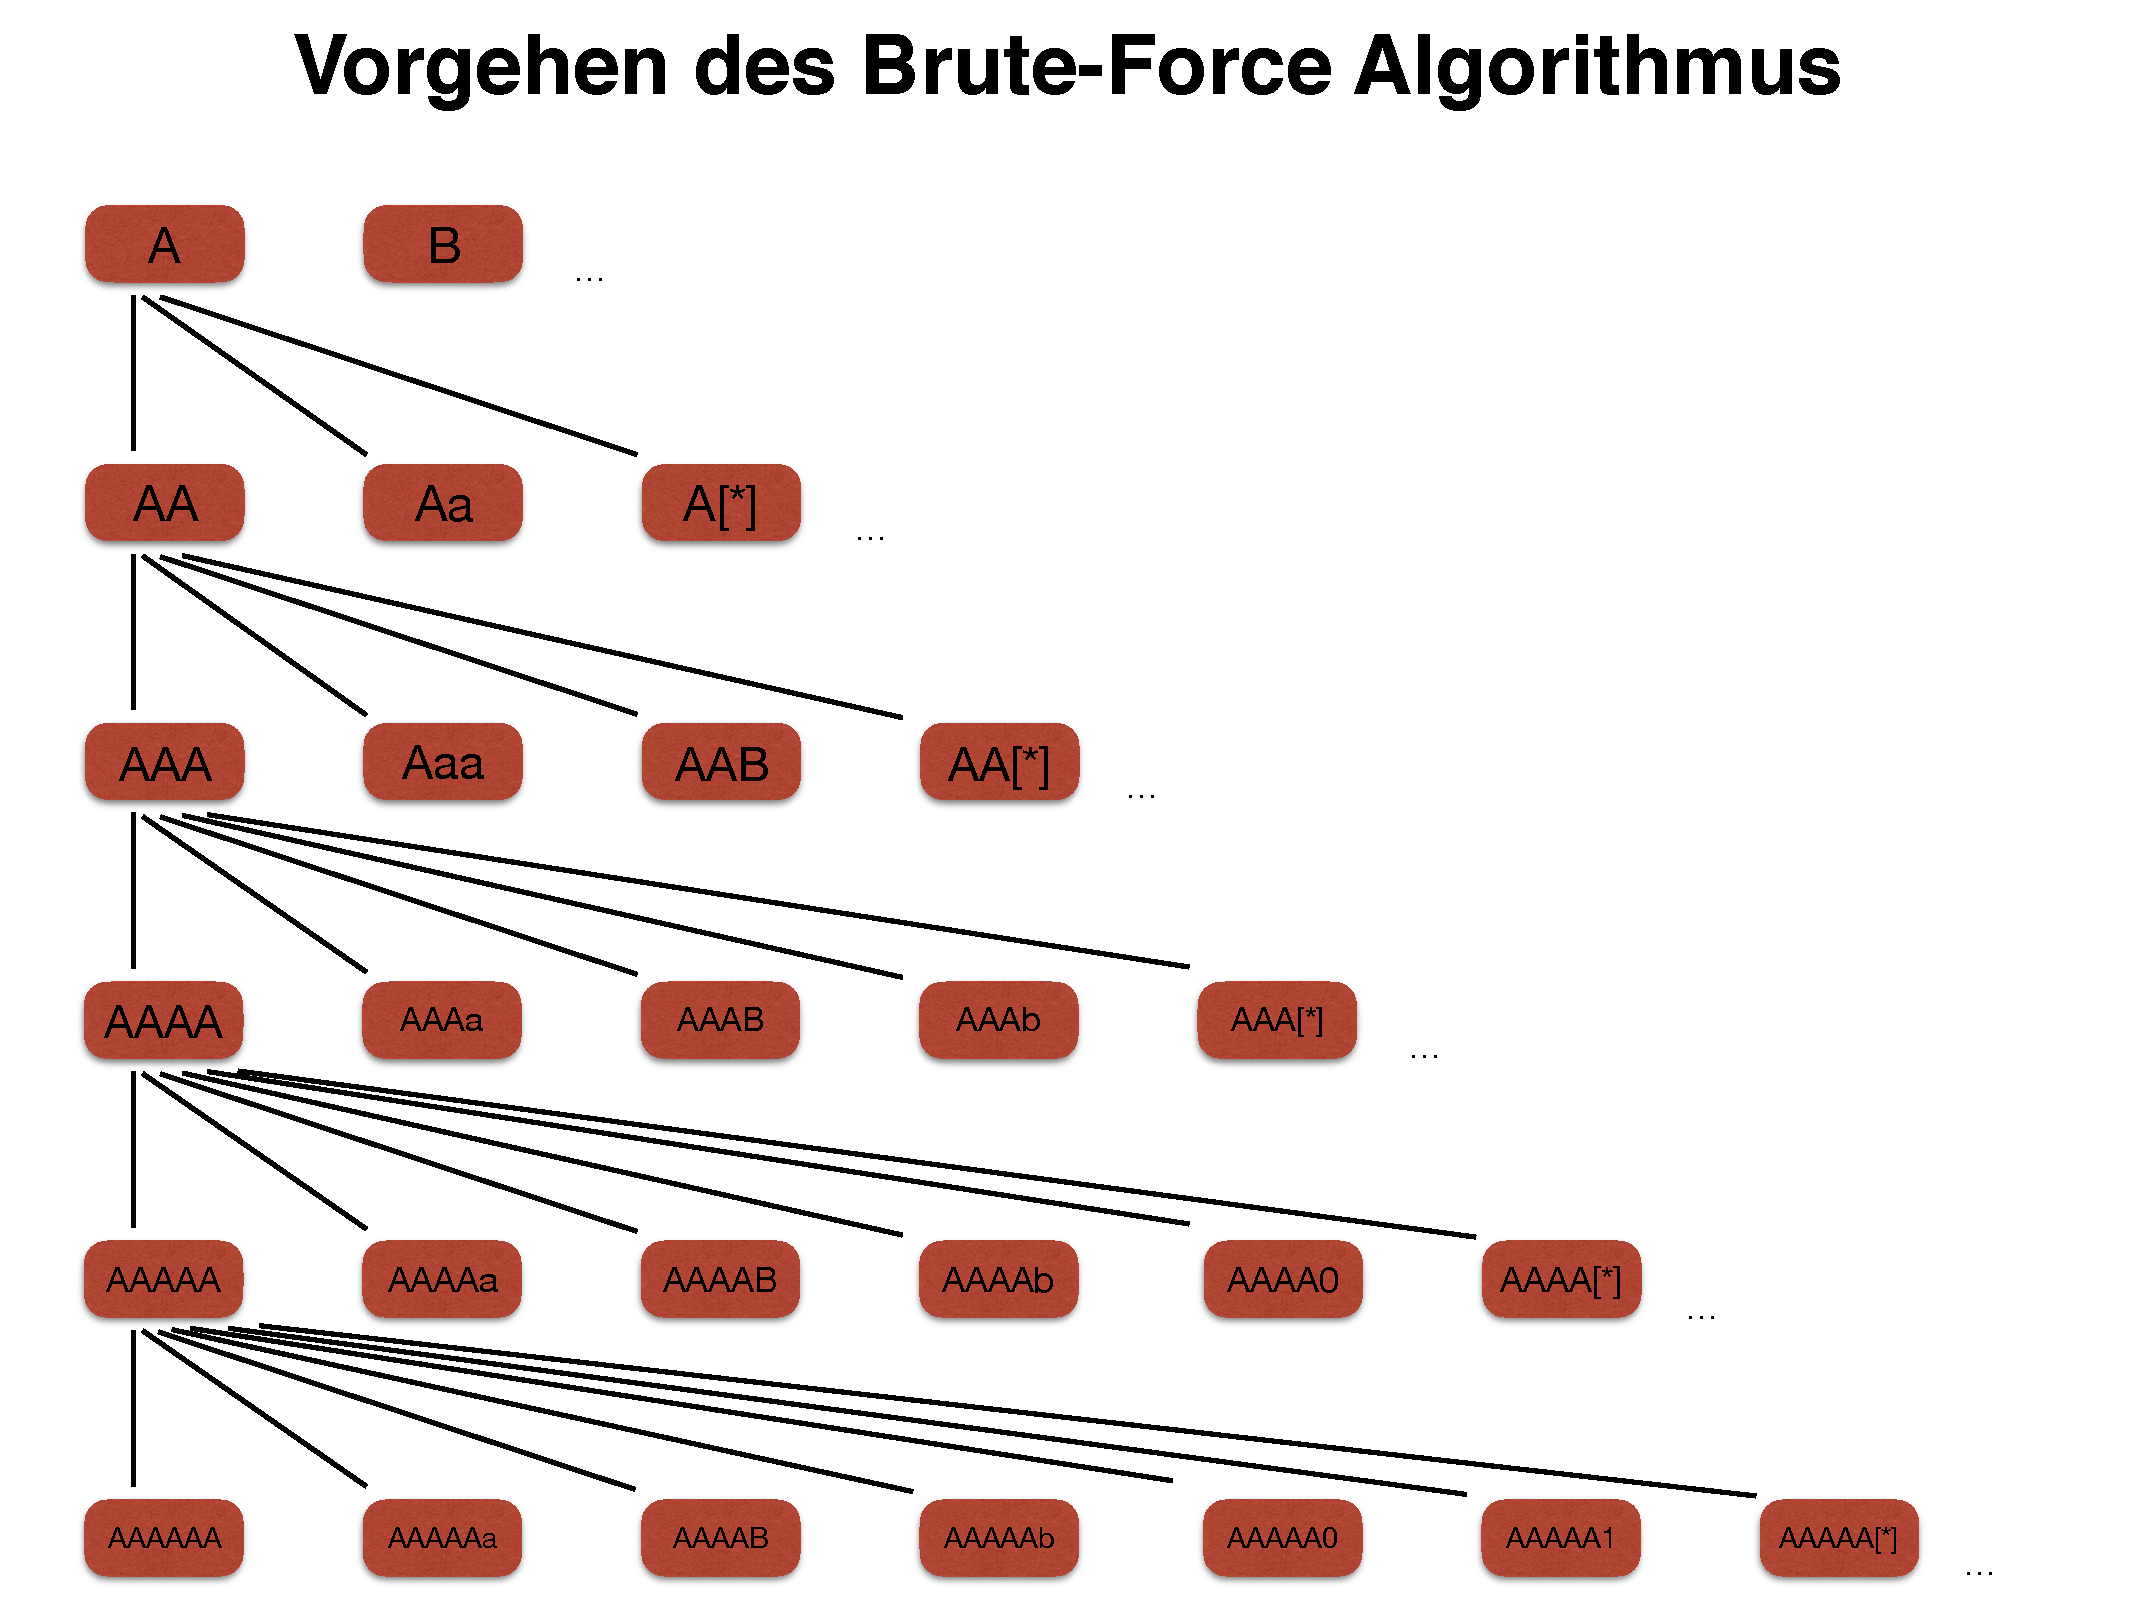
\includegraphics[natwidth=1200pt, natheight=349pt, width=1.0\textwidth]{images/SchaubildAlgorithmBreitensuche.pdf}
	\caption{Darstellung der Suchstrategie, die der Brute-Force Algorithmus zum Ermitteln des Passwortes benutzt.}
	\label{fig:schemaBruteForce}
\end{figure}

Die berechneten Passwörter sollen dann in eine Warteschlange geschrieben werden, sodass die Worker des verteilten Systems sich \enquote{Arbeitspakete} holen können. Ein solches Arbeitspaket beinhaltet eine Sammlung von Passwörtern. Die Worker berechnen dann die Hashes der Passwörter und vergleichen diese mit dem Zielhash.\\
 Berechnet ein Worker einen Hash, der mit dem Zielhash überein stimmt, so ist das gesuchte Passwort identifiziert.  


\section{Architektur des verteilten Systems}
Das verteilte System wird so konzipiert, dass die vier in Kapitel \ref{allgemeineAnforderungen} genannten Anforderungen umgesetzt werden können. Um dies zu realisieren, wird mit einer nachrichtenbasierten Architektur geplant. Die Rechner des verteilten Systems können so miteinander kommunizieren, ohne dass eine restriktive Anordnung notwendig ist. Dadurch wird die Skalierbarkeit sichergestellt. \\
Außerdem wird durch die nachrichtenbasierte Architektur sichergestellt, dass die Ressourcen innerhalb des verteilten Systems leicht verfügbar sind. \\
Im verteilten System übernimmt der Master die Verantwortlichkeit für die Kommunikation, sodass die Skalierbarkeit weiter verbessert wird. Es wird lediglich ein Master im System benötigt, die Menge der Worker ist irrelevant. Konkret wird der Master die Funktion des Webservers beinhalten, welcher für die Steuerung des Nachrichtenversands innerhalb des verteilten Systems verantwortlich ist. Die Verbindungen werden mit Hilfe von Websockets aufgebaut.\\
Die Nachrichten werden versandt und in einer Warteschlange (MessageQueue) gespeichert. Somit haben alle Rechner des verteilten Systems Zugriff auf alle Nachrichten. Je nach Inhalt der Nachricht (z.B. \enquote{Nachricht an Worker}) wird entschieden, wer die jeweiligen Nachrichten erhalten oder verarbeiten soll. 

In den folgenden Skizzen sind die Planungen auf konzeptioneller Ebene zusammengefasst.

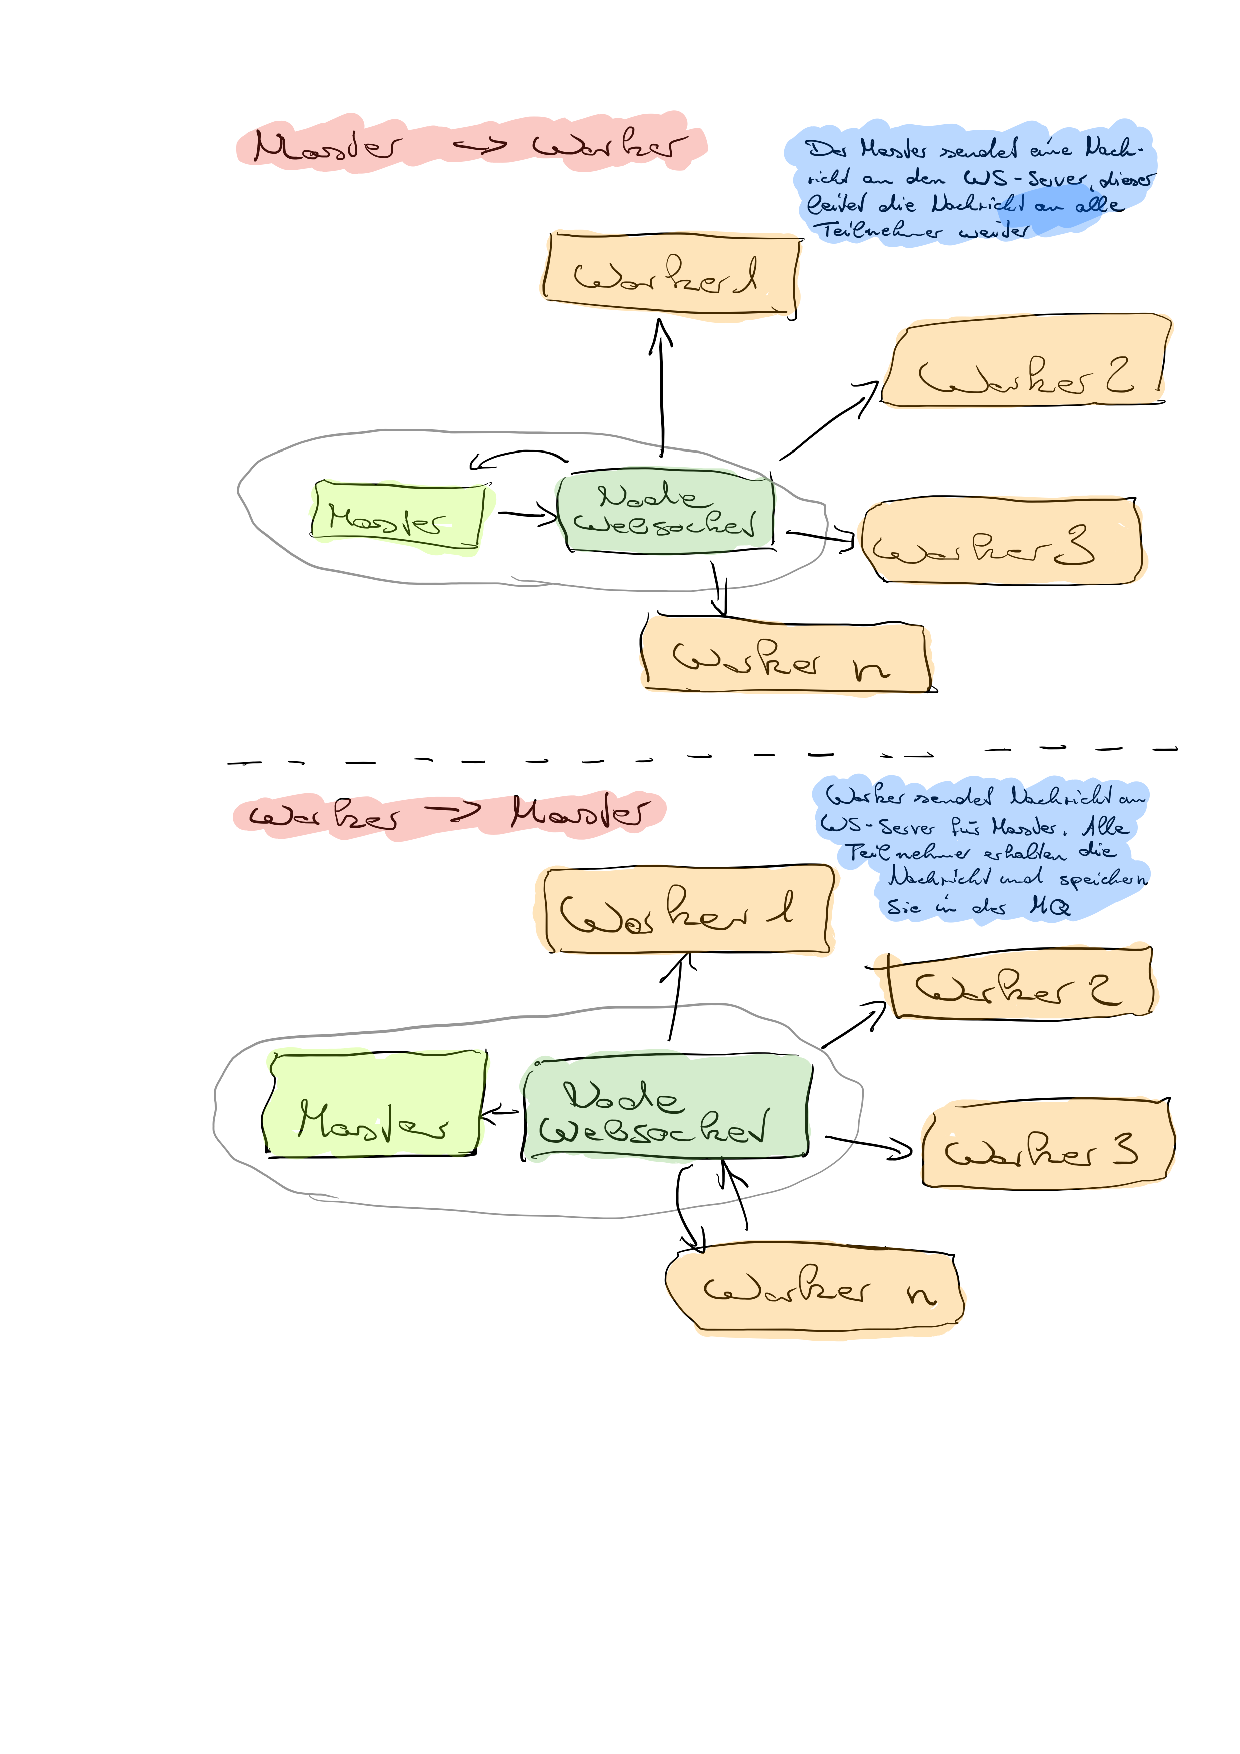
\includepdf[pages={1}]{images/systemarchitektur1.pdf}
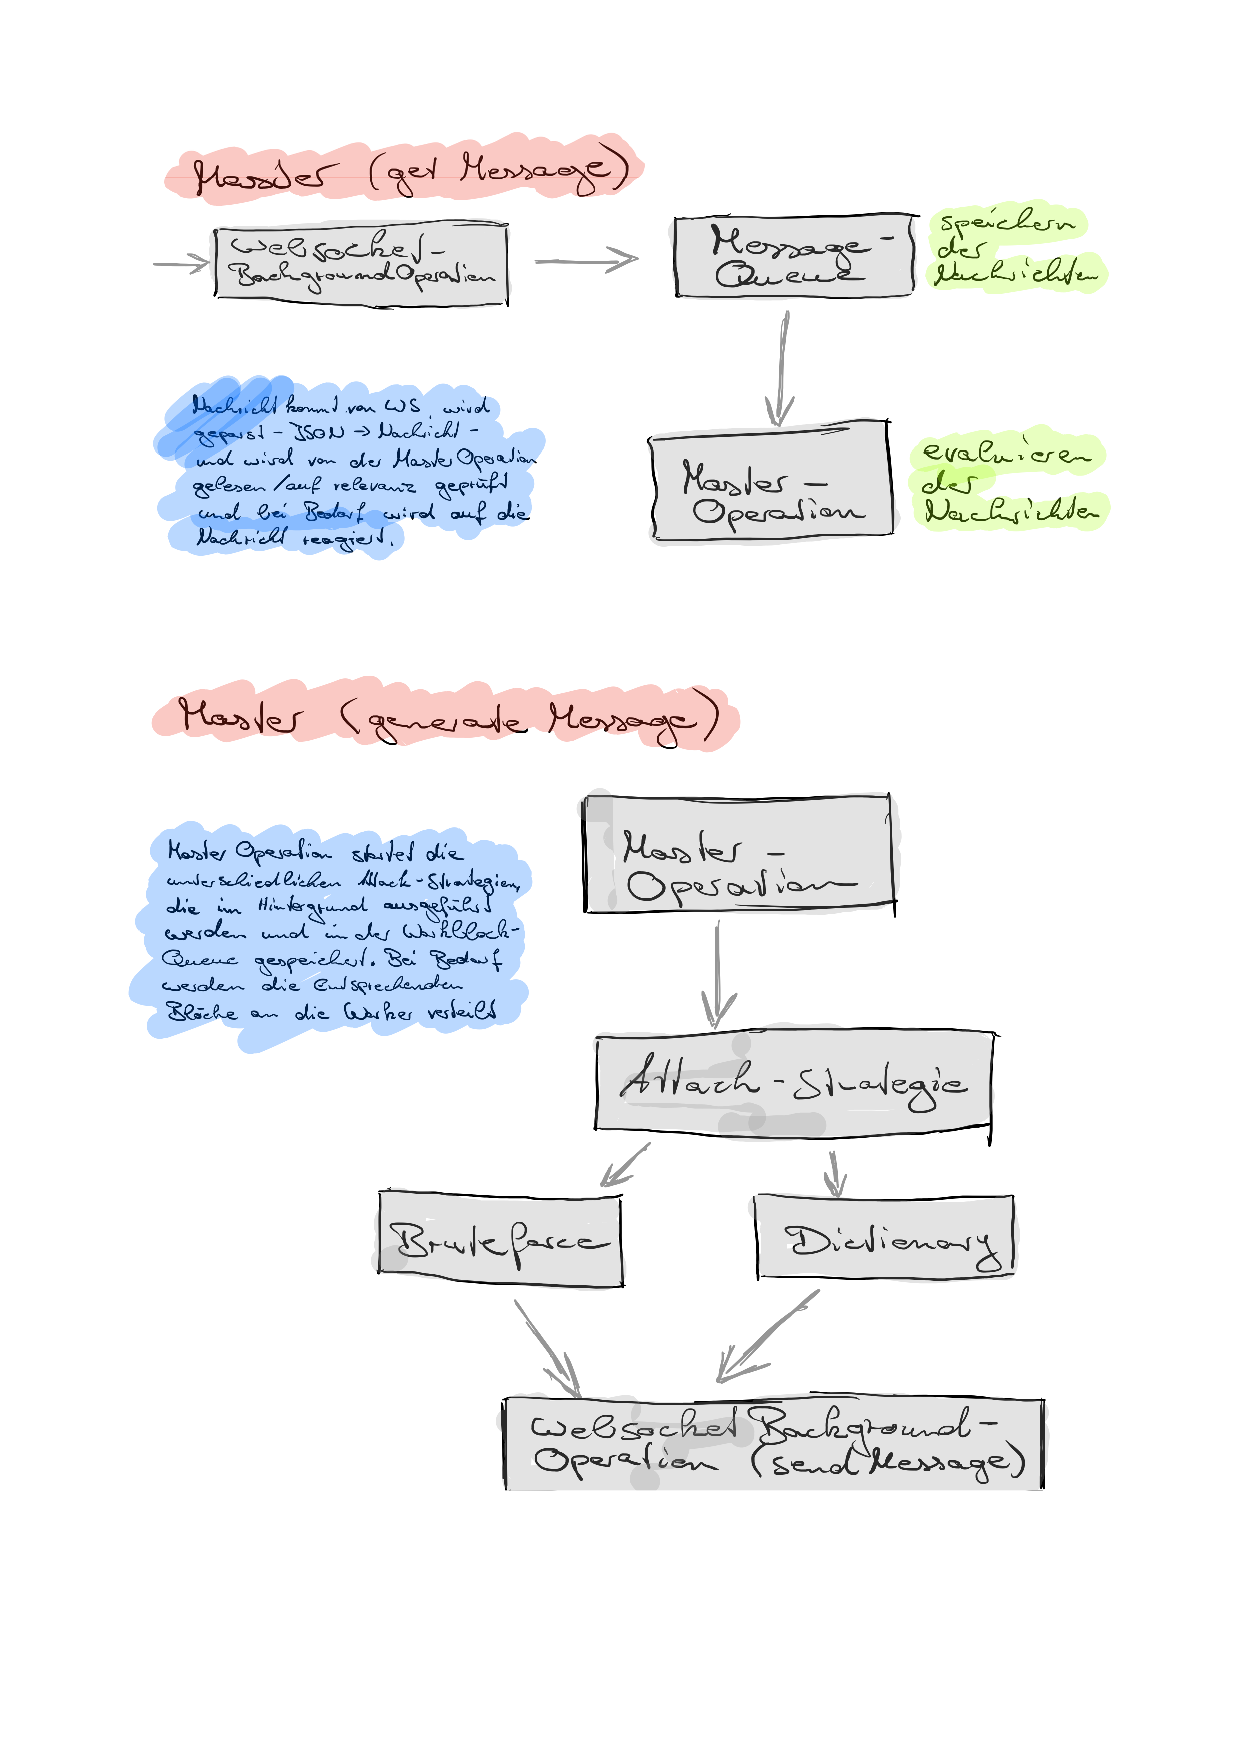
\includepdf[pages={1}]{images/systemarchitektur2.pdf}
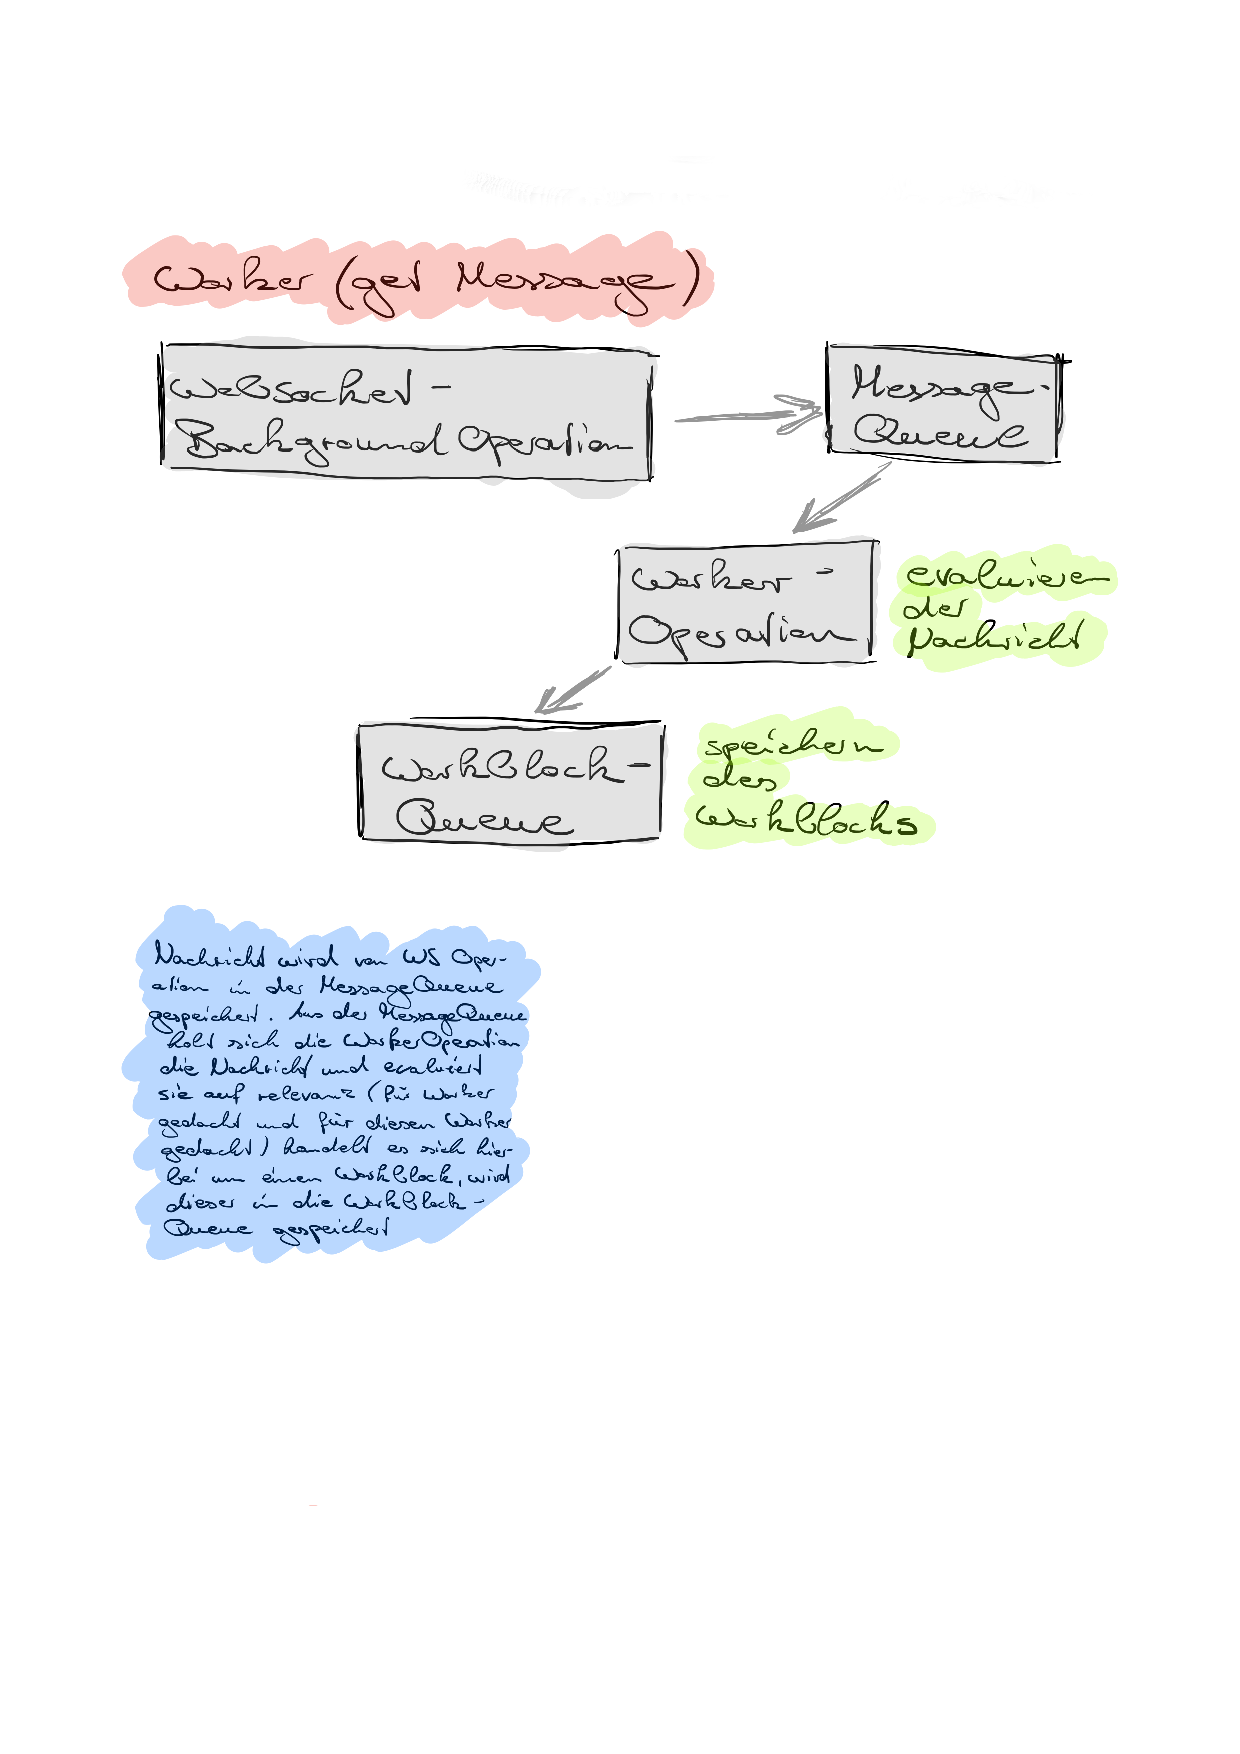
\includepdf[pages={1}]{images/systemarchitektur3.pdf}
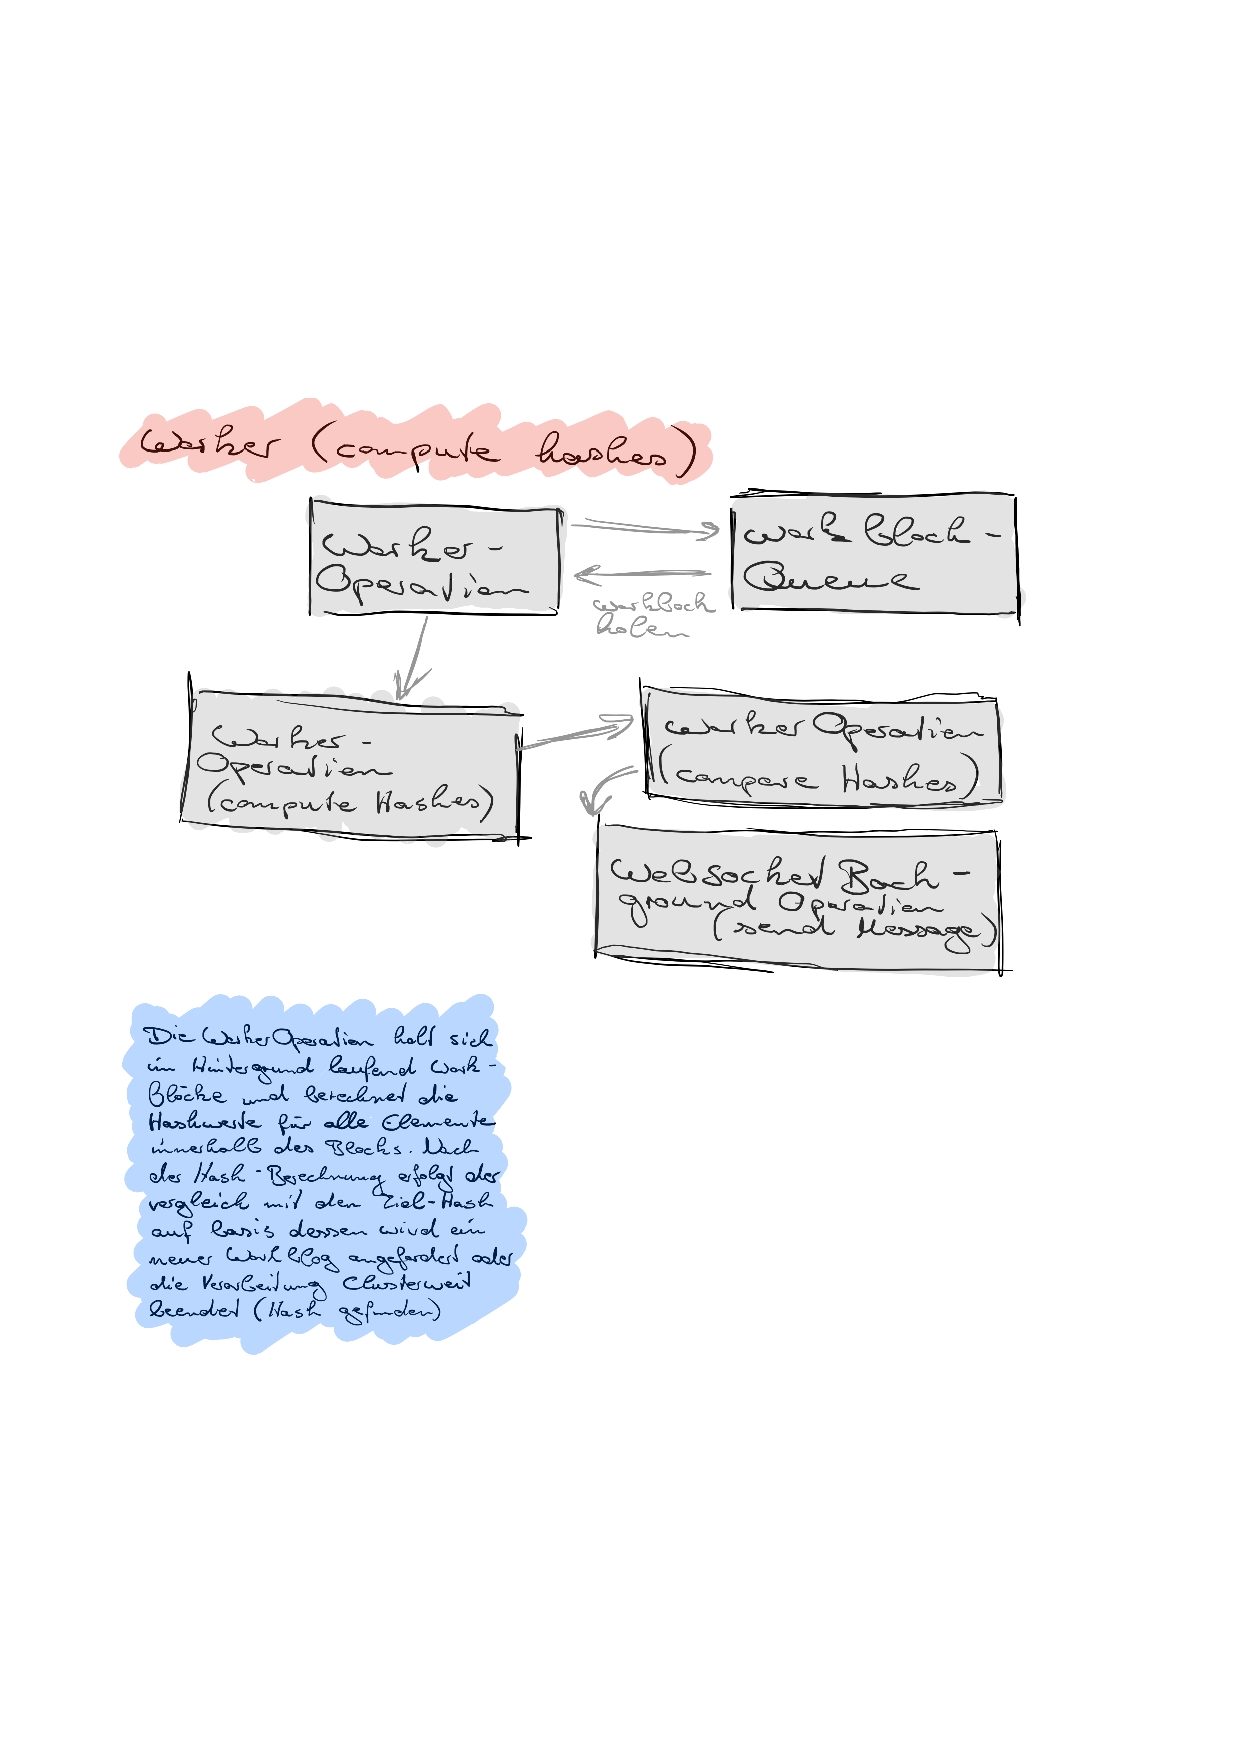
\includepdf[pages={1}]{images/systemarchitektur4.pdf}
